% vim:ts=2 sw=2 et spell tw=80:

\section{Construction of the Spherical Harmonics}

\kugeltodo{Review text, or rewrite if preliminaries becomes an addendum}

We finally arrived at the main section, which gives our chapter its name. The
idea is to discuss spherical harmonics, their mathematical derivation and some
of their properties and applications.

The subsection \ref{} \kugeltodo{Fix references} will be devoted to the
Eigenvalue problem of the Laplace operator. Through the latter we will derive
the set of Eigenfunctions that obey the equation presented in \ref{}
\kugeltodo{reference to eigenvalue equation}, which will be defined as
\emph{Spherical Harmonics}. In fact, this subsection will present their
mathematical derivation.

In the subsection \ref{}, on the other hand, some interesting properties
related to them will be discussed. Some of these will come back to help us
understand in more detail why they are useful in various real-world
applications, which will be presented in the section \ref{}.

One specific property will be studied in more detail in the subsection \ref{},
namely the recursive property.  The last subsection is devoted to one of the
most beautiful applications (In our humble opinion), namely the derivation of a
Fourier-style series expansion but defined on the sphere instead of a plane.
More importantly, this subsection will allow us to connect all the dots we have
created with the previous sections, concluding that Fourier is just a specific
case of the application of the concept of orthogonality. Our hope is that after
reading this section you will appreciate the beauty and power of generalization
that mathematics offers us.

\subsection{Eigenvalue Problem}
\label{kugel:sec:construction:eigenvalue}

\begin{figure}
  \centering
  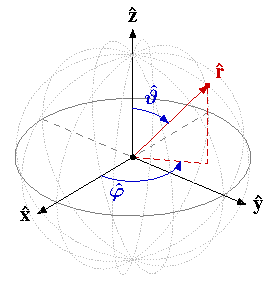
\includegraphics{papers/kugel/figures/tikz/spherical-coordinates}
  \caption{
    Spherical coordinate system. Space is described with the free variables $r
    \in \mathbb{R}_0^+$, $\vartheta \in [0; \pi]$ and $\varphi \in [0; 2\pi)$.
    \label{kugel:fig:spherical-coordinates}
  }
\end{figure}

From Section \ref{buch:pde:section:kugel}, we know that the spherical Laplacian
in the spherical coordinate system (shown in Figure
\ref{kugel:fig:spherical-coordinates}) is is defined as
\begin{equation*}
    \sphlaplacian :=
      \frac{1}{r^2} \frac{\partial}{\partial r} \left(
        r^2 \frac{\partial}{\partial r}
      \right)
      + \frac{1}{r^2} \left[
          \frac{1}{\sin\vartheta} \frac{\partial}{\partial \vartheta} \left(
            \sin\vartheta \frac{\partial}{\partial\vartheta}
          \right)
        + \frac{1}{\sin^2 \vartheta} \frac{\partial^2}{\partial\varphi^2}
      \right].
\end{equation*}
But we will not consider this algebraic monstrosity in its entirety. As the
title suggests, we will only care about the \emph{surface} of the sphere.  This
is for many reasons, but mainly to simplify reduce the already broad scope of
this text. Concretely, we will always work on the unit sphere, which just means
that we set $r = 1$ and keep only $\vartheta$ and $\varphi$ as free variables.
Now, since the variable $r$ became a constant, we can leave out all derivatives
with respect to $r$ and substitute all $r$'s with 1's to obtain a new operator
that deserves its own name.

\begin{definition}[Surface spherical Laplacian]
  \label{kugel:def:surface-laplacian}
  The operator
  \begin{equation*}
      \surflaplacian :=
        \frac{1}{\sin\vartheta} \frac{\partial}{\partial \vartheta} \left(
          \sin\vartheta \frac{\partial}{\partial\vartheta}
        \right)
        + \frac{1}{\sin^2 \vartheta} \frac{\partial^2}{\partial\varphi^2},
  \end{equation*}
  is called the surface spherical Laplacian.
\end{definition}

In the definition, the subscript ``$\partial S$'' was used to emphasize the
fact that we are on the spherical surface, which can be understood as being the
boundary of the sphere. But what does it actually do? To get an intuition,
first of all, notice the fact that $\surflaplacian$ have second derivatives,
which means that this a measure of \emph{curvature}; But curvature of what? To
get an even stronger intuition we will go into geometry, were curvature can be
grasped very well visually. Consider figure \ref{kugel:fig:curvature} where the
curvature is shown using colors. First we have the curvature of a curve in 1D,
then the curvature of a surface (2D), and finally the curvature of a function on
the surface of the unit sphere.

\begin{figure}
  \centering
  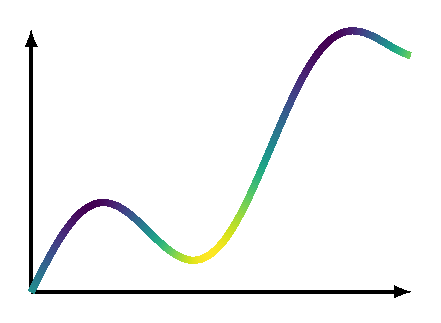
\includegraphics[width=.3\linewidth]{papers/kugel/figures/tikz/curvature-1d}
  \hskip 5mm
  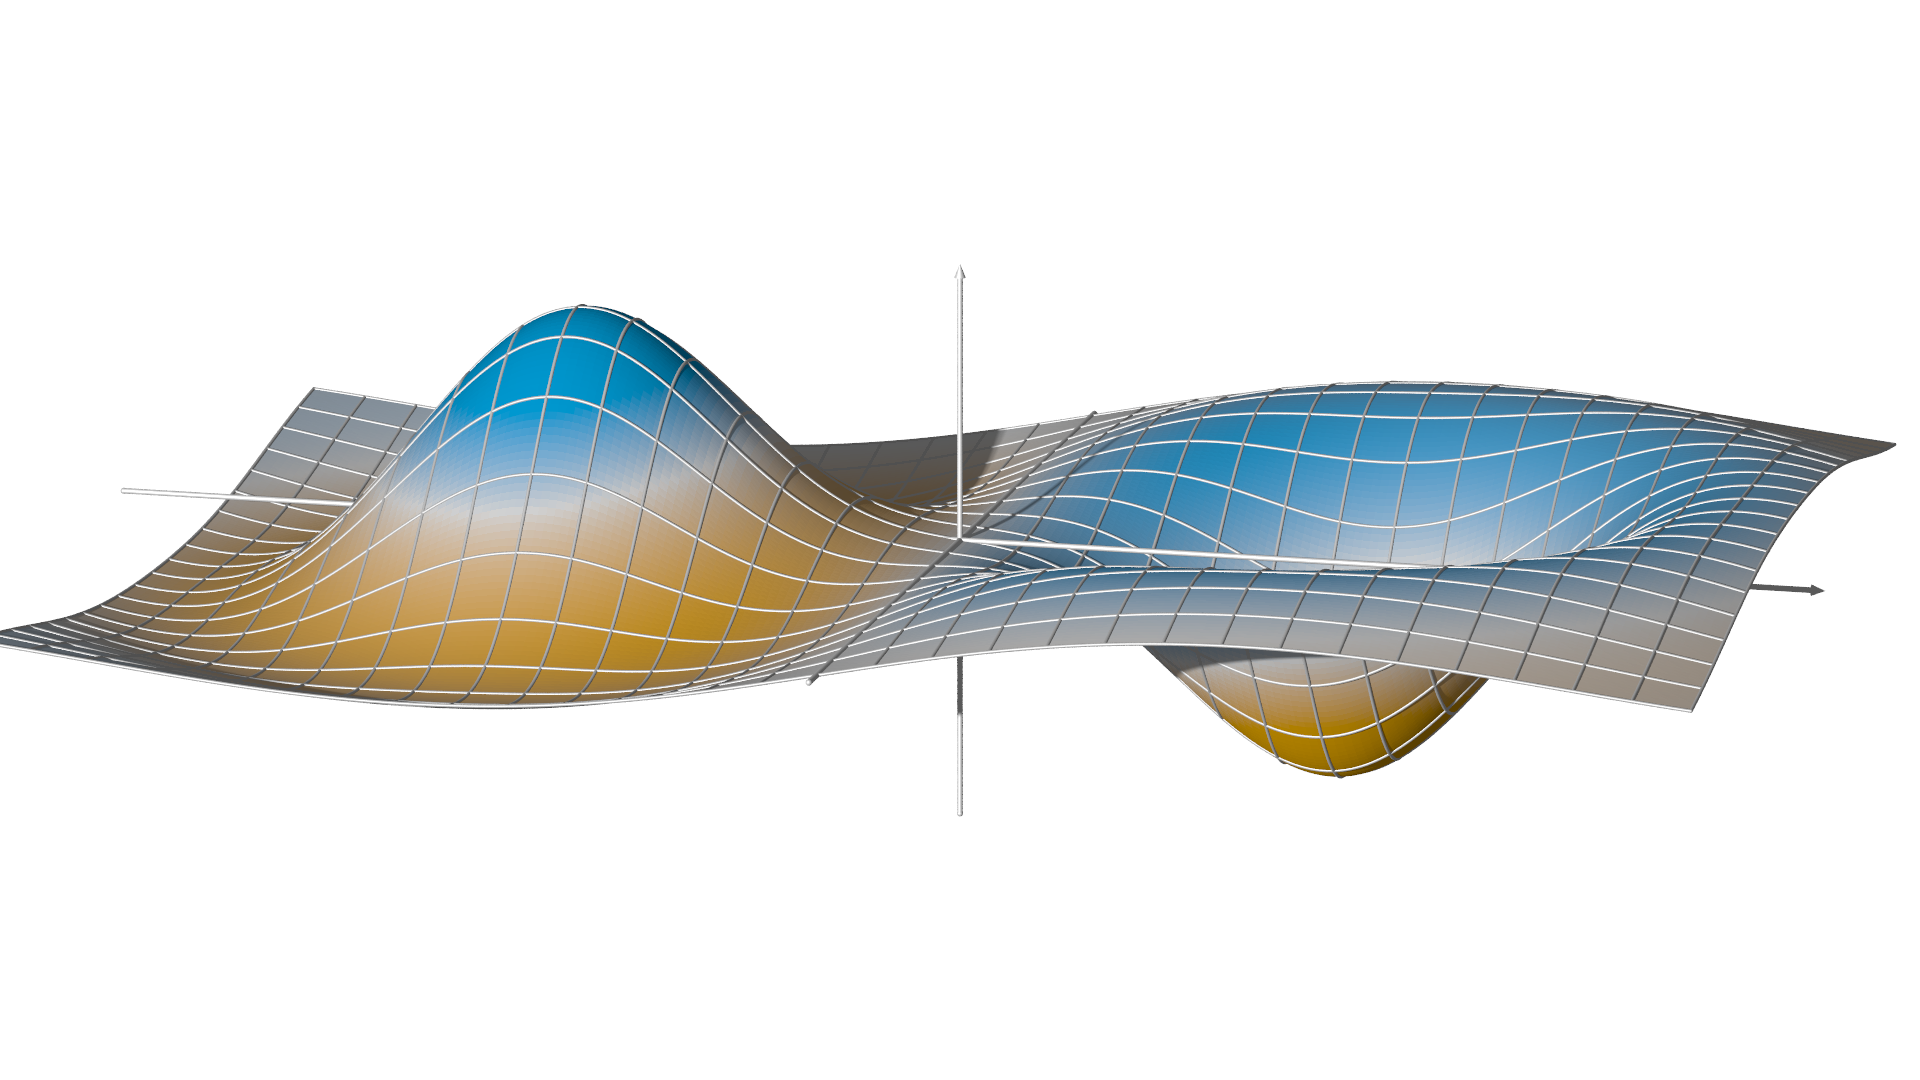
\includegraphics[width=.3\linewidth]{papers/kugel/figures/povray/curvature}
  \hskip 5mm
  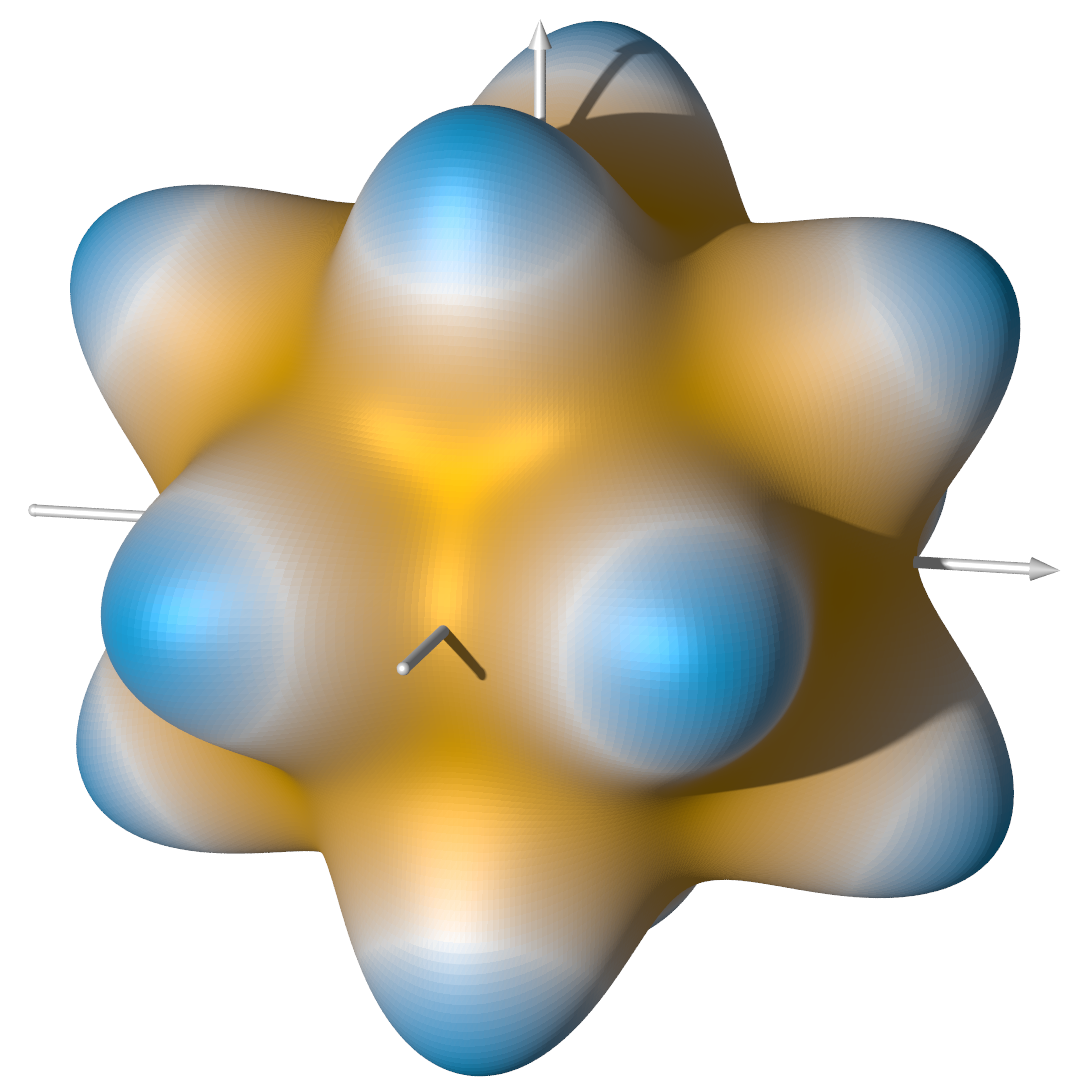
\includegraphics[width=.3\linewidth]{papers/kugel/figures/povray/spherecurve}
  \caption{
    \kugeltodo{Fix alignment / size, add caption. Would be nice to match colors.}
    \label{kugel:fig:curvature}
  }
\end{figure}

Now that we have defined an operator, we can go and study its eigenfunctions,
which means that we would like to find the functions $f(\vartheta, \varphi)$
that satisfy the equation
\begin{equation} \label{kugel:eqn:eigen}
    \surflaplacian f = -\lambda f.
\end{equation}
Perhaps it may not be obvious at first glance, but we are in fact dealing with a
partial differential equation (PDE) \kugeltodo{Boundary conditions?}. If we
unpack the notation of the operator $\nabla^2_{\partial S}$ according to
definition
\ref{kugel:def:surface-laplacian}, we get:
\begin{equation} \label{kugel:eqn:eigen-pde}
    \frac{1}{\sin\vartheta} \frac{\partial}{\partial \vartheta} \left(
      \sin\vartheta \frac{\partial f}{\partial\vartheta}
    \right)
    + \frac{1}{\sin^2 \vartheta} \frac{\partial^2 f}{\partial\varphi^2}
    + \lambda f = 0.
\end{equation}
Since all functions satisfying \eqref{kugel:eqn:eigen-pde} are the
\emph{eigenfunctions} of $\surflaplacian$, our new goal is to solve this PDE.
The task may seem very difficult but we can simplify it with a well-known
technique: \emph{the separation Ansatz}. It consists in assuming that the
function $f(\vartheta, \varphi)$ can be factorized in the following form:
\begin{equation}
    f(\vartheta, \varphi) = \Theta(\vartheta)\Phi(\varphi). 
\end{equation}
In other words, we are saying that the effect of the two independent variables
can be described using the multiplication of two functions that describe their
effect separately. This separation process was already presented in section
\ref{buch:pde:section:kugel}, but we will briefly rehearse it here for
convenience. If we substitute this assumption in
\eqref{kugel:eqn:eigen-pde}, we have:
\begin{equation*}
    \frac{1}{\sin\vartheta} \frac{\partial}{\partial \vartheta} \left(
      \sin\vartheta \frac{\partial  \Theta(\vartheta)}{\partial\vartheta}
    \right) \Phi(\varphi)
    + \frac{1}{\sin^2 \vartheta}
      \frac{\partial^2 \Phi(\varphi)}{\partial\varphi^2}
      \Theta(\vartheta)
    + \lambda \Theta(\vartheta)\Phi(\varphi) = 0.
\end{equation*}
Dividing by $\Theta(\vartheta)\Phi(\varphi)$ and introducing an auxiliary
variable $m^2$, the separation constant, yields:
\begin{equation*}
  \frac{1}{\Theta(\vartheta)}\sin \vartheta \frac{d}{d \vartheta} \left(
    \sin \vartheta \frac{d \Theta}{d \vartheta}
  \right)
  + \lambda \sin^2 \vartheta
  = -\frac{1}{\Phi(\varphi)} \frac{d^2\Phi(\varphi)}{d\varphi^2}
  = m^2,
\end{equation*}
which is equivalent to the following system of 2 first order differential
equations (ODEs):
\begin{subequations}
  \begin{gather}
    \frac{d^2\Phi(\varphi)}{d\varphi^2} = -m^2 \Phi(\varphi),
      \label{kugel:eqn:ode-phi} \\ 
    \sin \vartheta \frac{d}{d \vartheta} \left(
      \sin \vartheta \frac{d \Theta}{d \vartheta}
    \right)
    + \left( \lambda - \frac{m^2}{\sin^2 \vartheta} \right)
      \Theta(\vartheta) = 0
      \label{kugel:eqn:ode-theta}.
  \end{gather}
\end{subequations}
The solution of \eqref{kugel:eqn:ode-phi} is easy to find: The complex
exponential is obviously the function we are looking for. So we can directly
write the solutions
\begin{equation} \label{kugel:eqn:ode-phi-sol}
    \Phi(\varphi) = e^{i m \varphi}, \quad m \in \mathbb{Z}.
\end{equation}
The restriction that the separation constant $m$ needs to be an integer arises
from the fact that we require a $2\pi$-periodicity in $\varphi$ since the
coordinate systems requires that $\Phi(\varphi + 2\pi) = \Phi(\varphi)$.
Unfortunately, solving \eqref{kugel:eqn:ode-theta} is not as straightforward,
actually, it is quite difficult, and the process is so involved that it will
require a dedicated section of its own.

\subsection{Legendre Functions}

\begin{figure}
  \centering
  \kugelplaceholderfig{.8\textwidth}{5cm}
  \caption{
    \kugeltodo{Why $z = \cos \vartheta$.}
  }
\end{figure}

To solve \eqref{kugel:eqn:ode-theta} we start with the substitution $z = \cos
\vartheta$ \kugeltodo{Explain geometric origin with picture}. The operator
$\frac{d}{d \vartheta}$ becomes
\begin{equation*}
    \frac{d}{d \vartheta}
    = \frac{dz}{d \vartheta}\frac{d}{dz}
    = -\sin \vartheta \frac{d}{dz}
    = -\sqrt{1-z^2} \frac{d}{dz},
\end{equation*} 
since $\sin \vartheta = \sqrt{1 - \cos^2 \vartheta} = \sqrt{1 - z^2}$, and
then \eqref{kugel:eqn:ode-theta} becomes 
\begin{align*}
  \frac{-\sqrt{1-z^2}}{\sqrt{1-z^2}} \frac{d}{dz} \left[
    \left(\sqrt{1-z^2}\right) \left(-\sqrt{1-z^2}\right) \frac{d \Theta}{dz}
  \right]
  + \left( \lambda - \frac{m^2}{1 - z^2} \right)\Theta(\vartheta) &= 0,
  \\
  \frac{d}{dz} \left[ (1-z^2) \frac{d \Theta}{dz} \right]
  + \left( \lambda - \frac{m^2}{1 - z^2} \right)\Theta(\vartheta) &= 0,
  \\
  (1-z^2)\frac{d^2 \Theta}{dz} - 2z\frac{d \Theta}{dz}
  + \left( \lambda - \frac{m^2}{1 - z^2} \right)\Theta(\vartheta) &= 0.
\end{align*}
By making two final cosmetic substitutions, namely $Z(z) = \Theta(\cos^{-1}z)$
and $\lambda = n(n+1)$, we obtain what is known in the literature as the
\emph{associated Legendre equation of order $m$}:
\nocite{olver_introduction_2013}
\begin{equation} \label{kugel:eqn:associated-legendre}
  (1 - z^2)\frac{d^2 Z}{dz^2}
  - 2z\frac{d Z}{dz}
  + \left( n(n + 1) - \frac{m^2}{1 - z^2} \right) Z(z) = 0,
  \quad
  z \in [-1; 1], m \in \mathbb{Z}.
\end{equation}

Our new goal has therefore become to solve
\eqref{kugel:eqn:associated-legendre}, since if we find a solution for $Z(z)$ we
can perform the substitution backwards and get back to our eigenvalue problem.
However, the associated Legendre equation is not any easier, so to attack the
problem we will look for the solutions in the easier special case when $m = 0$.
This reduces the problem because it removes the double pole, which is always
tricky to deal with. In fact, the reduced problem when $m = 0$ is known as the
\emph{Legendre equation}:
\begin{equation} \label{kugel:eqn:legendre}
  (1 - z^2)\frac{d^2 Z}{dz^2}
  - 2z\frac{d Z}{dz}
  + n(n + 1) Z(z) = 0,
  \quad
  z \in [-1; 1].
\end{equation}

The Legendre equation is a second order differential equation, and therefore it
has 2 independent solutions, which are known as \emph{Legendre functions} of the
first and second kind. For the scope of this text we will only derive a special
case of the former that is known known as the \emph{Legendre polynomials}, since
we only need a solution between $-1$ and $1$.

\begin{lemma}[Legendre polynomials]
  \label{kugel:thm:legendre-poly}
  The polynomial function
  \[
    P_n(z) = \sum^{\lfloor n/2 \rfloor}_{k=0}
      \frac{(-1)^k}{2^n s^k!} \frac{(2n - 2k)!}{(n - k)! (n-2k)!} z^{n - 2k}
  \]
  is the only finite solution of the Legendre equation
  \eqref{kugel:eqn:legendre} when $n \in \mathbb{Z}$ and $z \in [-1; 1]$.
\end{lemma}
\begin{proof}
  This results is derived in section \ref{kugel:sec:proofs:legendre}.
\end{proof}

Since the Legendre \emph{polynomials} are indeed polynomials, they can also be
expressed using the hypergeometric functions described in section
\ref{buch:rekursion:section:hypergeometrische-funktion}, so in fact
\begin{equation}
  P_n(z) = {}_2F_1 \left( \begin{matrix}
    n + 1, & -n \\ \multicolumn{2}{c}{1}
  \end{matrix} ; \frac{1 - z}{2} \right).
\end{equation}
Further, there are a few more interesting but not very relevant forms to write
$P_n(z)$ such as \emph{Rodrigues' formula} and \emph{Laplace's integral
representation} which are
\begin{equation*}
  P_n(z) = \frac{1}{2^n n!} \frac{d^n}{dz^n} (z^2 - 1)^n,
  \qquad \text{and} \qquad
  P_n(z) = \frac{1}{\pi} \int_0^\pi \left(
    z + \cos\vartheta \sqrt{z^2 - 1}
  \right) \, d\vartheta
\end{equation*}
respectively, both of which we will not prove (see chapter 3 of
\cite{bell_special_2004} for a proof). Now that we have a solution for the
Legendre equation, we can make use of the following lemma patch the solutions
such that they also become solutions of the associated Legendre equation
\eqref{kugel:eqn:associated-legendre}.

\begin{lemma} \label{kugel:thm:extend-legendre}
  If $Z_n(z)$ is a solution of the Legendre equation \eqref{kugel:eqn:legendre},
  then
  \begin{equation*}
    Z^m_n(z) = (1 - z^2)^{m/2} \frac{d^m}{dz^m}Z_n(z)
  \end{equation*}
  solves the associated Legendre equation \eqref{kugel:eqn:associated-legendre}.
  \nocite{bell_special_2004}
\end{lemma}
\begin{proof}
  See section \ref{kugel:sec:proofs:legendre}.
\end{proof}

What is happening in lemma \ref{kugel:thm:extend-legendre}, is that we are
essentially inserting a square root function in the solution in order to be able
to reach the parts of the domain near the poles at $\pm 1$ of the associated
Legendre equation, which is not possible only using power series
\kugeltodo{Reference book theory on extended power series method.}. Now, since
we have a solution in our domain, namely $P_n(z)$, we can insert it in the lemma 
obtain the \emph{associated Legendre functions}.

\begin{definition}[Ferrers or associated Legendre functions]
  \label{kugel:def:ferrers-functions}
  The functions
  \begin{equation}
    P^m_n (z) = (1-z^2)^{\frac{m}{2}}\frac{d^{m}}{dz^{m}} P_n(z)
      = \frac{1}{2^n n!}(1-z^2)^{\frac{m}{2}}\frac{d^{m+n}}{dz^{m+n}}(1-z^2)^n, \quad |m|<n
  \end{equation}
  are known as Ferrers or associated Legendre functions.
\end{definition}
The constraint $|m|<n$, can be justified by considering Eq.\eqref{kugel:eq:associated_leg_func}, in which the derivative of degree $m+n$ is present. A derivative to be well defined must have an order that is greater than zero. Furthermore, it can be seen that this derivative is applied on a polynomial of degree $2n$. As is known from Calculus 1, if you derive a polynomial of degree $2n$ more than $2n$ times, you get zero, which is a trivial solution in which we are not interested.

We can thus summarize these two conditions by writing:
\begin{equation*}
    \begin{rcases}
        m+n \leq 2n &\implies m \leq n \\
        m+n \geq 0  &\implies  m \geq -n
    \end{rcases} \; |m| \leq n.
\end{equation*}
\if 0
The set of functions in Eq.\eqref{kugel:eq:sph_harm_0} is named \emph{Spherical Harmonics}, which are the eigenfunctions of the Laplace operator on the \emph{spherical surface domain}, which is exactly what we were looking for at the beginning of this section.
\fi

\subsection{Spherical Harmonics}

Finally, we can go back to solving our boundary value problem we started in
section \ref{kugel:sec:construction:eigenvalue}. We had left off in the middle
of the separation, were we had used the Ansatz $f(\vartheta, \varphi) =
\Theta(\vartheta) \Phi(\varphi)$ to find that $\Phi(\varphi) = e^{im\varphi}$,
and we were solving for $\Theta(\vartheta)$.  As you may recall, previously we
performed the substitution $z = \cos \vartheta$. Now we can finally to bring back the
solution to the associated Legendre equation $P^m_n(z)$ into the $\vartheta$
domain and combine it with $\Phi(\varphi)$ to get the full result:
\begin{equation*}
    f(\vartheta, \varphi)
      = \Theta(\vartheta)\Phi(\varphi)
      = P^m_n (\cos \vartheta) e^{im\varphi}, \quad |m|<n.
\end{equation*}
This family of functions, which recall are the solutions of the eigenvalue
problem of the surface spherical Laplacian, are the long anticipated
\emph{complex spherical harmonics}, and they are usually denoted with
$Y^m_n(\vartheta, \varphi)$.

\begin{definition}[Spherical harmonics]
  \label{kugel:def:spherical-harmonics}
  The functions
  \begin{equation*}
    Y^m_n (\vartheta, \varphi) = P^m_n(\cos \vartheta) e^{im\varphi}, \quad |m|<n
  \end{equation*}
  where $m, n \in \mathbb{Z}$ are called (unnormalized) spherical
  harmonics.
\end{definition}

\begin{figure}
  \centering
  \kugelplaceholderfig{\textwidth}{.8\paperheight}
  \caption{
    \kugeltodo{Big picture with the first few spherical harmonics.}
    \label{kugel:fig:spherical-harmonics}
  }
\end{figure}

\kugeltodo{Describe how they look like with fig.
\ref{kugel:fig:spherical-harmonics}}

\subsection{Orthogonality of $P_n$, $P^m_n$ and $Y^m_n$}

We shall now discuss an important property of the spherical harmonics: they form
an orthogonal system. And since the spherical harmonics contain the Ferrers or
associated Legendre functions, we need to discuss their orthogonality first.
But the Ferrers functions themselves depend on the Legendre polynomials, so that
will be our starting point.

\begin{lemma} For the Legendre polynomials $P_n(z)$ and $P_k(z)$ it holds that
  \label{kugel:thm:legendre-poly-ortho}
  \begin{equation*}
    \int_{-1}^1 P_n(z) P_k(z) \, dz
    = \frac{2}{2n + 1} \delta_{nk}
    = \begin{cases}
      \frac{2}{2n + 1} & \text{if } n = k, \\
      0 & \text{otherwise}.
    \end{cases}
  \end{equation*}
\end{lemma}
\begin{proof}
  To start, consider the fact that the Legendre equation
  \eqref{kugel:eqn:legendre}, of which two distinct Legendre polynomials
  $P_n(z)$ and $P_k(z)$ are a solution ($n \neq k$), can be rewritten in the
  following form:
  \begin{equation}
    \frac{d}{dz} \left[ 
      \left( 1 - z^2 \right) \frac{dZ}{dz}
    \right] + n(n+1) Z(z) = 0.
  \end{equation}
  So we rewrite the Legendre equations for $P_n(z)$ and $P_k(z)$:
  \begin{align*}
    \frac{d}{dz} \left[ 
      \left( 1 - z^2 \right) \frac{dP_n}{dz}
    \right] + n(n+1) P_n(z) &= 0,
    &
    \frac{d}{dz} \left[ 
      \left( 1 - z^2 \right) \frac{dP_k}{dz}
    \right] + k(k+1) P_k(z) &= 0,
  \end{align*}
  then we multiply the former by $P_k(z)$ and the latter by $P_n(z)$ and
  subtract the two to get
  \begin{equation*}
    \frac{d}{dz} \left[ 
      \left( 1 - z^2 \right) \frac{dP_n}{dz}
    \right] P_k(z) + n(n+1) P_n(z) P_k(z)
    -
    \frac{d}{dz} \left[ 
      \left( 1 - z^2 \right) \frac{dP_k}{dz}
    \right] P_n(z) - k(k+1) P_k(z) P_n(z) = 0.
  \end{equation*}
  By grouping terms, making order and integrating with respect to $z$ from $-1$
  to 1 we obtain
  \begin{gather}
    \int_{-1}^1 \left\{
      \frac{d}{dz} \left[ 
        \left( 1 - z^2 \right) \frac{dP_n}{dz}
      \right] P_k(z) 
      -
      \frac{d}{dz} \left[ 
        \left( 1 - z^2 \right) \frac{dP_k}{dz}
      \right] P_n(z) - k(k+1) P_k(z) P_n(z)
    \right\} \,dz \nonumber \\
    + \left[ n(n+1) - k(k+1) \right] \int_{-1}^1 P_k(z) P_n(z) \, dz = 0.
    \label{kugel:thm:legendre-poly-ortho:proof:1}
  \end{gather}
  Since by the product rule
  \begin{equation*}
    \frac{d}{dz} \left[ (1 - z^2) \frac{dP_k}{dz} P_n(z) \right]
    =
    \frac{d}{dz} \left[ (1 - z^2) \frac{dP_n}{dz} \right] P_k(z)
      + (1 - z^2) \frac{dP_n}{dz} \frac{dP_k}{dz},
  \end{equation*}
  we can simplify the first term in
  \eqref{kugel:thm:legendre-poly-ortho:proof:1} to get
  \begin{gather*}
    \int_{-1}^1 \left\{
      \frac{d}{dz} \left[ (1 - z^2) \frac{dP_k}{dz} P_n(z) \right]
        - \cancel{(1 - z^2) \frac{dP_n}{dz} \frac{dP_k}{dz}}
        - \frac{d}{dz} \left[ (1 - z^2) \frac{dP_n}{dz} P_k(z) \right]
        + \cancel{(1 - z^2) \frac{dP_k}{dz} \frac{dP_n}{dz}}
    \right\} \, dz \\
    = \int_{-1}^1 \frac{d}{dz} \left\{ (1 - z^2) \left[
      \frac{dP_k}{dz} P_n(z) - \frac{dP_n}{dz} P_k(z)
    \right] \right\} \, dz
    = (1 - z^2) \left[
      \frac{dP_k}{dz} P_n(z) - \frac{dP_n}{dz} P_k(z)
    \right] \Bigg|_{-1}^1,
  \end{gather*}
  which always equals 0 because the product contains $1 - z^2$ and the bounds
  are at $\pm 1$. Thus, of \eqref{kugel:thm:legendre-poly-ortho:proof:1} only
  the second term remains and the equation becomes
  \begin{equation*}
    \left[ n(n+1) - k(k+1) \right] \int_{-1}^1 P_k(z) P_n(z) \, dz = 0.
  \end{equation*}
  By dividing by the constant in front of the integral we have our first result.
  Now we need to show that when $n = k$ the integral equals $2 / (2n + 1)$.
  % \begin{equation*}
  % \end{equation*}
  \kugeltodo{Finish proof. Can we do it without the generating function of
  $P_n$?}
\end{proof}

In a similarly algebraically tedious fashion, we can also continue to check for
orthogonality for the Ferrers functions $P^m_n(z)$, since they are related to
$P_n(z)$ by a $m$-th derivative, and obtain the following result.

\begin{lemma} For the associated Legendre functions
  \label{kugel:thm:associated-legendre-ortho}
  \begin{equation*}
    \int_{-1}^1 P^m_n(z) P^{m}_{n'}(z) \, dz
    = \frac{2(m + n)!}{(2n + 1)(n - m)!} \delta_{nn'}
    = \begin{cases}
      \frac{2(m + n)!}{(2n + 1)(n - m)!}
        & \text{if } n = n', \\
      0 & \text{otherwise}.
    \end{cases}
  \end{equation*}
\end{lemma}
\begin{proof}
  To show that the expression equals zero when $n \neq n'$ we can perform
  exactly the same steps as in the proof of lemma
  \ref{kugel:thm:legendre-poly-ortho}, so we will not repeat them here and prove
  instead only the case when $n = n'$.
  \kugeltodo{Finish proof, or not? I have to look and decide if it is
  interesting enough.}
\end{proof}

By having the orthogonality relations of the Legendre functions we can finally
show that spherical harmonics are also orthogonal under the following inner
product:

\begin{definition}[Inner product in $S^2$]
  \label{kugel:def:inner-product-s2}
  For 2 complex valued functions $f(\vartheta, \varphi)$ and $g(\vartheta,
  \varphi)$ on the surface of the sphere the inner product is defined to be
  \begin{equation*}
    \langle f, g \rangle
    = \int_{0}^\pi \int_0^{2\pi}
      f(\vartheta, \varphi) \overline{g(\vartheta, \varphi)}
      \sin \vartheta \, d\varphi \, d\vartheta.
  \end{equation*}
\end{definition}


\begin{theorem} For the (unnormalized) spherical harmonics
  \label{kugel:thm:spherical-harmonics-ortho}
  \begin{align*}
    \langle Y^m_n, Y^{m'}_{n'} \rangle
    &= \int_{0}^\pi \int_0^{2\pi}
      Y^m_n(\vartheta, \varphi) \overline{Y^{m'}_{n'}(\vartheta, \varphi)}
      \sin \vartheta \, d\varphi \, d\vartheta
    \\
    &= \frac{4\pi}{2n + 1} \frac{(m + n)!}{(n - m)!} \delta_{nn'} \delta_{mm'}
    = \begin{cases}
      \frac{4\pi}{2n + 1} \frac{(m + n)!}{(n - m)!}
        & \text{if } n = n' \text{ and } m = m', \\
      0 & \text{otherwise}.
    \end{cases}
  \end{align*}
\end{theorem}
\begin{proof}
  We will begin by doing a bit of algebraic maipulaiton:
  \begin{align*}
    \int_{0}^\pi \int_0^{2\pi}
      Y^m_n(\vartheta, \varphi) \overline{Y^{m'}_{n'}(\vartheta, \varphi)}
      \sin \vartheta \, d\varphi \, d\vartheta
    &= \int_{0}^\pi \int_0^{2\pi}
      e^{im\varphi} P^m_n(\cos \vartheta)
      e^{-im'\varphi} P^{m'}_{n'}(\cos \vartheta)
      \, d\varphi \sin \vartheta \, d\vartheta
    \\
    &= \int_{0}^\pi
      P^m_n(\cos \vartheta) P^{m'}_{n'}(\cos \vartheta)
      \int_0^{2\pi} e^{i(m - m')\varphi}
      \, d\varphi \sin \vartheta \, d\vartheta
      .
  \end{align*}
  First, notice that the associated Legendre polynomials are assumed to be real,
  and are thus unaffected by the complex conjugation. Then, we can see that when
  $m = m'$ the inner integral simplifies to $\int_0^{2\pi} 1 \, d\varphi$ which
  equals $2\pi$, so in this case the expression becomes
  \begin{equation*}
    2\pi \int_{0}^\pi
      P^m_n(\cos \vartheta) P^{m'}_{n'}(\cos \vartheta)
    \sin \vartheta \, d\vartheta
    = -2\pi \int_{1}^{-1} P^m_n(z) P^{m'}_{n'}(z) \, dz
    = \frac{4\pi(m + n)!}{(2n + 1)(n - m)!} \delta_{nn'},
  \end{equation*}
  where in the second step we performed the substitution $z = \cos\vartheta$;
  $d\vartheta = \frac{d\vartheta}{dz} dz= - dz / \sin \vartheta$, and then we
  used lemma \ref{kugel:thm:associated-legendre-ortho}. We are allowed to use
  the lemma because $m = m'$.

  Now we just need look at the case when $m \neq m'$. Fortunately this is
  easier: the inner integral is $\int_0^{2\pi} e^{i(m - m')\varphi} d\varphi$,
  or in other words we are integrating a complex exponetial over the entire
  period, which always results in zero. Thus, we do not need to do anything and
  the proof is complete.
\end{proof}

These proofs for the various orthogonality relations were quite long and
algebraically tedious, mainly because they are ``low level'', by which we mean
that they (arguably) do not rely on very abstract theory. However, if we allow
ourselves to use the more abstract Sturm Liouville theory discussed in chapters
\ref{buch:integrale:subsection:sturm-liouville-problem} and \kugeltodo{reference
to chapter 17 of haddouche and Löffler} the proofs can become ridiculously
short. Let's do for example lemma \ref{kugel:thm:associated-legendre-ortho}.

\begin{proof}[
    Shorter proof of lemma \ref{kugel:thm:associated-legendre-ortho}
  ]
  The associated Legendre polynomials, of which we would like to prove an
  orthogonality relation, are the solution to the associated Legendre equation,
  which we can write as $LZ(z) = 0$, where
  \begin{equation*}
    L = \frac{d}{dz} (1 - z^2) \frac{d}{dz}
      + n(n+1) - \frac{m^2}{1 - z^2}.
  \end{equation*}
  Notice that $L$ is in fact a Sturm-Liouville operator of the form
  \begin{equation*}
    L = \frac{1}{w(z)} \left[
        \frac{d}{dz} p(z) \frac{d}{dz} - \lambda + q(z)
      \right],
  \end{equation*}
  if we let $w(z) = 1$, $p(z) = (1 - z^2 )$, $q(z) = -m^2 / (1 - z^2)$, and
  $\lambda = -n(n+1)$. By the theory of Sturm-Liouville operators, we know that
  the each solution of the problem $LZ(z) = 0$, namely $P^m_n(z)$, is orthogonal
  to every other solution that has a different $\lambda$. In our case $\lambda$
  varies with $n$, so $P^m_n(z)$ with different $n$'s are orthogonal to each
  other.
\end{proof}

But that was still rather informative and had a bit of explanation, which is
terrible. Real snobs, such as Wikipedia contributors, some authors and
regrettably sometimes even ourselves, would write instead:

\begin{proof}[
    Infuriatingly short proof of lemma \ref{kugel:thm:associated-legendre-ortho}
  ]
  The associated Legendre polynomials are solutions of the associated Legendre
  equation which is a Sturm-Liouville problem and are thus orthogonal to each
  other. The factor in front Kronecker delta is left as an exercise to the
  reader.
\end{proof}

Lemma \ref{kugel:thm:legendre-poly-ortho} has a very similar
proof, while the theorem \ref{kugel:thm:spherical-harmonics-ortho} for the
spherical harmonics is proved by the following argument. The spherical harmonics
are the solutions to the eigenvalue problem $\surflaplacian f = -\lambda f$,
which as discussed in the previous section is solved using separation. So to
prove their orthogonality using the Sturm-Liouville theory we argue that
\begin{equation*}
  \surflaplacian = L_\vartheta L_\varphi \iff
  \surflaplacian f(\vartheta, \varphi)
    = L_\vartheta \Theta(\vartheta) L_\varphi \Phi(\varphi),
\end{equation*}
then we show that both $L_\vartheta$ and $L_\varphi$ are both Sturm-Liouville
operators (we just did the former in the shorter proof above). Since both are
Sturm-Liouville operators their combination, the surface spherical Laplacian, is
also a Sturm-Liouville operator, which then implies orthogonality.

\subsection{Normalization and the Phase Factor}

At this point we have shown that the spherical harmonics form an orthogonal
system, but in many applications we usually also want a normalization of some
kind. For example the most obvious desirable property could be for the spherical
harmonics to be ortho\emph{normal}, by which we mean that $\langle Y^m_n,
Y^{m'}_{n'} \rangle = \delta_{nn'}$. To obtain orthonormality, we simply add an
ugly normalization factor in front of the previous definition
\ref{kugel:def:spherical-harmonics} as follows.

\begin{definition}[Orthonormal spherical harmonics]
  \label{kugel:def:spherical-harmonics-orthonormal}
  The functions
  \begin{equation*}
    Y^m_n(\vartheta, \varphi)
    = \sqrt{\frac{2n + 1}{4\pi} \frac{(n-m)!}{(m+n)!}}
      P^m_n(\cos \vartheta) e^{im\varphi}
  \end{equation*}
  where $m, n \in \mathbb{Z}$ and $|m| < n$ are the orthonormal spherical
  harmonics.
\end{definition}

Orthornomality is very useful, but it is not the only common normalization that
is found in the literature. In physics, geomagnetism to be more specific, it is
common to use the so called Schmidt semi-normalization (or sometimes also called
quasi-normalization).

\begin{definition}[Schmidt semi-normalized spherical harmonics]
  \label{kugel:def:spherical-harmonics-schmidt}
  The Schmidt semi-normalized spherical harmonics are
  \begin{equation*}
    Y^m_n(\vartheta, \varphi)
    = \sqrt{2 \frac{(n - m)!}{(n + m)!}}
      P^m_n(\cos \vartheta) e^{im\varphi}
  \end{equation*}
  where $m, n \in \mathbb{Z}$ and $|m| < n$.
\end{definition}

Additionally, there is another quirk in the literature that should be mentioned.
In some other branches of physics such as seismology and quantum mechanics there
is a so called Condon-Shortley phase factor $(-1)^m$ in front of the square root
in the definition of the normalized spherical harmonics. It is yet another
normalization that is added for physical reasons that are not very relevant to
our discussion, but we mention this potential source of confusion since many
numerical packages (such as \texttt{SHTOOLS} \kugeltodo{Reference}) offer an
option to add or remove it from the computation.

Though, for our purposes we will mostly only need the orthonormal spherical
harmonics, so from now on, unless specified otherwise when we say spherical
harmonics or write $Y^m_n$, we mean the orthonormal spherical harmonics of
definition \ref{kugel:def:spherical-harmonics-orthonormal}.

\subsection{Recurrence Relations}
The idea of this subsection is to introduce first some recursive relations regarding the Associated Legendre Functions, defined in eq.\eqref{kugel:def:ferrers-functions}. Subsequently we will extend them, in order to derive recurrence formulas for the case of Spherical Harmonic functions as well. 
\subsubsection{Associated Legendre Functions}
To start this journey, we can first write the following equations, which relate the Associated Legendre functions of different indeces $m$ and $n$ recursively:
\begin{enumerate}[(i)]
  \item $(2n+1) x P^m_n(z)= (m+n) P^m_{n-1}(z) + (n-m+1) P^m_{n+1}(z)$, \label{kugel:eq:rec_rel_1}
  \item $\dfrac{2mz}{\sqrt{1-z^2}} P^m_n(z) = P^{m+1}_n(z) + [n(n+1)-m(m-1)] P^{m-1}_n(z)$, \label{kugel:eq:rec_rel_2}
  \item $\sqrt{1-z^2} P^m_n(z) = \dfrac{1}{2n+1} \left[ P^{m+1}_{n+1}(z) - P^{m+1}_{n-1}(z) \right]$,  \label{kugel:eq:rec_rel_3}
  \item $\sqrt{1-z^2} P^m_n(z) = \dfrac{1}{2n+1} \left[ (n+m)(n+m-1)P^{m-1}_{n-1}(z) - (n-m+1)(n-m+2)P^{m-1}_{n+1}(z) \right]$.  \label{kugel:eq:rec_rel_4}
\end{enumerate}
Much of the effort will be proving this bunch of equalities. Then, in the second part, where we will derive the recursion equations for $Y^m_n(\vartheta,\varphi)$, we will basically reuse the ones presented above.

Maybe it is worth mentioning at least one use case for these relations: They are widely used in some software implementations, as they lead to better numerical accuracy and computational cost lower by a factor of six\cite{usecase_recursion}.
\begin{enumerate}[(i)]
  \item 
  \begin{proof}
    This is the relation that links the associated Legendre functions with the same $m$ index but different $n$. Using \ref{} \kugeltodo{ref alla recurrence dei polinomi di legendre (è da qualche parte nel libro)}, we have 
    \begin{equation*}
      (n+1)P_{n+1}(z)-(2n+1)xP_n(z)+nP_{n-1}(z)=0,
    \end{equation*}
    that can be differentiated $m$ times, obtaining
    \begin{equation}\label{kugel:eq:rec_1}
      (n+1)\frac{d^mP_{n+1}}{dz^m}-(2n+1) \left[z \frac{d^m P_n}{dz^m}+ m\frac{d^{m-1}P_{n-1}}{dz^{m-1}} \right] + n\frac{d^m P_{n-1}}{dz^m}=0.
    \end{equation}
    To continue this derivation, we need the following relation:
    \begin{equation}\label{kugel:eq:rec_2}
      \frac{dP_{n+1}}{dz} - \frac{dP_{n-1}}{dz} = (2n+1)P_n.
    \end{equation}
    The latter will not be derived, because it suffices to use the definition of the Legendre Polynomials $P_n(x)$ to check it.
    
    We can now differentiate the just presented eq.\eqref{kugel:eq:rec_2} $m-1$ times, that will become
    \begin{equation}\label{kugel:eq:rec_3}
      \frac{d^mP_{n+1}}{dx^m} - \frac{d^mP_{n-1}}{dx^m} = (2n+1)\frac{d^{m-1}P_n}{dx^{m-1}}.
    \end{equation}
    Then, using eq.\eqref{kugel:eq:rec_3} in eq.\eqref{kugel:eq:rec_1}, we will have
    \begin{equation}\label{kugel:eq:rec_4}
      (n+1)\frac{d^mP_{n+1}}{dx^m}- (2n+1)\frac{d^mP_{n+1}}{dx^m} -m\left[\frac{d^m P_{n+1}}{dx^m}+ \frac{d^{m}P_{n-1}}{dx^m}\right] + n\frac{d^m P_{n-1}}{dx^m}=0.
    \end{equation}
    Finally, multiplying both sides by $(1-x^2)^{\frac{m}{2}}$ and simplifying the expression, we can rewrite eq.\eqref{kugel:eq:rec_4} in terms of $P^m_n(x)$, namely
    \begin{equation*}
      (n+1-m)P^m_{n+1}(x)-(2n+1)xP^m_n(x)+(m+n)P^m_{n-1}(x)=0,
    \end{equation*}
    that rearranged, will be
    \begin{equation*}
      (2n+1) x P^m_n(x)= (m+n) P^m_{n-1}(x) + (n-m+1) P^m_{n+1}(x).
    \end{equation*}
  \end{proof}
  
  \item
  \begin{proof}
    This relation, unlike the previous one, link three expression with the same $n$ index but different $m$. 
    
    In the proof of Lemma \ref{kugel:lemma:sol_associated_leg_eq}, at some point we ran into this expression.
    \begin{equation*}
      (1-x^2)\frac{d^{m+2}P_n}{dx^{m+2}} - 2(m+1)x \frac{d^{m+1}P_n}{dx^{m+1}} + [n(n+1)-m(m+1)]\frac{d^mP_n}{dx^m} = 0,
    \end{equation*}
    that, if multiplied by $(1-x^2)^{\frac{m}{2}}$, will be
    \begin{equation*}
      (1-x^2)^{\frac{m}{2}+1}\frac{d^{m+2}P_n}{dx^{m+2}} - 2(m+1)x (1-x^2)^{\frac{m}{2}}\frac{d^{m+1}P_n}{dx^{m+1}} + [n(n+1)-m(m+1)](1-x^2)^{\frac{m}{2}}\frac{d^mP_n}{dx^m} = 0.
    \end{equation*}
    Therefore, as before, expressing it in terms of $P^m_n(x)$:
    \begin{equation*}
      P^{m+2}_n(x) - \frac{2(m+1)x}{\sqrt{1-x^2}}P^{m+1}_n(x) + [n(n+1)-m(m+1)]P^m_n(x)=0.
    \end{equation*}
    Furthermore, we can adjust the indeces and terms, obtaining
    \begin{equation*}
      \frac{2mx}{\sqrt{(1-x^2)}} P^m_n(x) = P^{m+1}_n(x) + [n(n+1)-m(m-1)] P^{m-1}_n(x)
    \end{equation*}
  
  \end{proof}
  
  \item
  \begin{proof}
    To derive this expression, we can multiply eq.\eqref{kugel:eq:rec_3} by $(1-x^2)^{\frac{m}{2}}$ and, as always, we could express it in terms of $P^m_n(x)$:
    \begin{equation*}
      P^m_{n+1}(x) - P^m_{n-1}(x) = (2n+1)\sqrt{1-x^2}P^{m-1}_n(x).
    \end{equation*}
    Afer that we can divide by $2n+1$ resulting in
    \begin{equation}\label{kugel:eq:helper}
      \frac{1}{2n+1}[P^m_{n+1}(x) - P^m_{n-1}(x)] = \sqrt{1-x^2}P^{m-1}_n(x).
    \end{equation}
    To conclude, we arrange the indeces differently:
    \begin{equation*}
      \sqrt{1-x^2}P^{m}_n(x)=\frac{1}{2n+1}[P^{m+1}_{n+1}(x) - P^{m+1}_{n-1}(x)].
    \end{equation*}
  \end{proof}

  \item
  \begin{proof}
    For this proof we can rely on (\ref{kugel:eq:rec_rel_1}), and therefore rewrite (\ref{kugel:eq:rec_rel_2}) as 
    \begin{equation*}
      \frac{2m}{(2n+1)\sqrt{1-x^2}} \left[ (m+n)P^m_{n-1}(x) + (n-m+1)P^m_{n+1}(x) \right] = P^{m+1}_n(x) + [ n(n+1)-m(m-1) ]P^{m-1}_n(x).
    \end{equation*}
    Rewriting then $P^{m-1}_n(x)$ using eq.\eqref{kugel:eq:helper}, we will have
    \begin{align*}
      \frac{2m}{(2n+1)\sqrt{1-x^2}} &\left[ (m+n)P^m_{n-1}(x) + (n-m+1)P^m_{n+1}(x) \right] = P^{m+1}_n(x) \\
      &+ \frac{n(n+1)-m(m-1)}{(2n+1)\sqrt{1-x^2}} \left[ P^m_{n+1}(x)-P^m_{n-1}(x) \right].
    \end{align*}
    The last equation, after some algebric rearrangements, it is easy to show that it is equivalent to
    \begin{equation*}
      \sqrt{1-x^2} P^m_n(x) = \dfrac{1}{2n+1} \left[ (n+m)(n+m-1)P^{m-1}_{n-1}(x) - (n-m+1)(n-m+2)P^{m-1}_{n+1}(x) \right]
    \end{equation*}
  \end{proof}

\end{enumerate}

\subsubsection{Spherical Harmonics}
The goal of this subsection's part is to apply the recurrence relations of the $P_n(z)$ functions to the Spherical Harmonics. 

With some little adjustments we will be able to have recursion equations for them too. As previously written the most of the work is already done. Now it is only a matter of minor mathematical operations/rearrangements.

We can start by listing all of them:
\begin{enumerate}[(i)]
  \item $Y^m_n(\vartheta, \varphi) = \dfrac{1}{(2n+1)\cos \vartheta} \left[ (m+n)Y^m_{n-1}(\vartheta, \varphi) + (m-n+1)Y^m_{n+1}(\vartheta, \varphi) \right]$
  \begin{proof}
    We can multiply both sides of equality in eq.\eqref{} by $e^{im \varphi}$ and perform the substitution $z=\cos \vartheta$. After a few simple algebraic steps, we will obtain the relation we are looking for
  \end{proof}
  \item $Y^m_n(\vartheta, \varphi) = \dfrac{\tan \vartheta}{2m}\left[ Y^{m+1}_n(\vartheta, \varphi)e^{-i\varphi} + [n(n+1)-m(m-1)]Y^{m-1}_n(\vartheta, \varphi)e^{i\varphi} \right]$
  \begin{proof}
    In this proof, as before, we can perform the substitution $z=\cos \vartheta$, and notice that $\sqrt{1-z^2}=\sin \vartheta$, hence, the relation in eq.\eqref{} will be
    \begin{equation*}
      \frac{2m \cos \vartheta}{\sin \vartheta} P^m_n(\cos \vartheta) =  P^{m+1}_n(\cos \vartheta) + [n(n+1)-m(m-1)]P^{m-1}_n P^m_n(\cos \vartheta).
    \end{equation*}
    The latter, multiplied by $e^{im\varphi}$, becomes
    \begin{align*}
      \frac{2m \cos \vartheta}{\sin \vartheta} P^m_n(\cos \vartheta)e^{im\varphi} &=  P^{m+1}_n(\cos \vartheta)e^{im\varphi} + [n(n+1)-m(m-1)]P^{m-1}_n P^m_n(\cos \vartheta)e^{im\varphi} \\
      &= P^{m+1}_n(\cos \vartheta)e^{i(m+1)\varphi}e^{-i\varphi} + [n(n+1)-m(m-1)]P^{m-1}_n (\cos \vartheta)e^{i(m-1)\varphi}e^{i\varphi} \\
      &= Y^{m+1}_n(\vartheta, \varphi)e^{-i\varphi} + [n(n+1)-m(m-1)]Y^{m-1}_n(\vartheta, \varphi)e^{i\varphi} \\
    \end{align*}
    Finally, after some ``cleaning''
    \begin{equation*}
      Y^m_n(\vartheta, \varphi) = \frac{\tan \vartheta}{2m} \left[ Y^{m+1}_n(\vartheta, \varphi)e^{-i\varphi} + [n(n+1)-m(m-1)]Y^{m-1}_n(\vartheta, \varphi)e^{i\varphi} \right]
    \end{equation*}
  \end{proof}
  \item $Y^m_n(\vartheta, \varphi) = \dfrac{e^{-i\varphi}}{ (2n+1)\sin \vartheta } \left[ Y^{m+1}_{n+1}(\vartheta, \varphi) - Y^{m+1}_{n-1}(\vartheta, \varphi) \right]$
  \begin{proof}
    Now we can consider eq.\eqref{}, and multiply it by $e^{im\varphi}$. After the usual substitution $z=\cos \vartheta$, we have 
    \begin{align*}
      \sin \vartheta P^m_n(\cos \vartheta)e^{im\varphi} &= \dfrac{e^{im\varphi}}{2n+1}\left[ P^{m+1}_{n+1}(\cos \vartheta) - P^{m+1}_{n-1}(\cos \vartheta)\right] \\
      &= \dfrac{e^{-i\varphi}}{2n+1}\left[ P^{m+1}_{n+1}(\cos \vartheta)e^{i(m+1)\varphi} - P^{m+1}_{n-1}(\cos \vartheta)e^{i(m+1)\varphi}\right] \\
    \end{align*}
    A few manipulations later, we will obtain
    \begin{equation*}
      Y^m_n(\vartheta, \varphi) = \frac{e^{-i\varphi}}{(2n+1)\sin \vartheta} \left[ Y^{m+1}_{n+1}(\vartheta, \varphi)-Y^{m+1}_{n-1}(\vartheta, \varphi) \right]
    \end{equation*}
  \end{proof}
  \item $Y^m_n(\vartheta, \varphi) = \dfrac{e^{i\varphi}}{(2n+1)\sin \vartheta} \left[ (n+m)(n+m-1)Y^{m-1}_{n-1}(\vartheta, \varphi) - (n-m+1)(n-m+2)Y^{m-1}_{n+1}(\vartheta, \varphi) \right]$
  \begin{proof}
    This proof is very similar to the previous one. We just have to perform the substitution $z = \cos \vartheta$, as always. Secondly we can multiply the right side by $e^{im\varphi}$ and the left one too but in a different form, namely $e^{im\varphi}=e^{i(m-1)\varphi}e^{i\varphi}$. Then it is only a question of recalling the definition of $Y^m_n(\vartheta, \varphi)$.
  \end{proof}
\end{enumerate}

\section{Series Expansions in $L^2(S^2)$}

We have now reached a point were we have all of the tools that are necessary to
build something truly amazing: a general series expansion formula for functions
on the surface of the sphere. Using the jargon: we will now see that the
spherical harmonics together with the inner product of definition
\ref{kugel:def:inner-product-s2}
\begin{equation*}
  \langle f, g \rangle
  = \int_{0}^\pi \int_0^{2\pi}
    f(\vartheta, \varphi) \overline{g(\vartheta, \varphi)}
    \sin \vartheta \, d\varphi \, d\vartheta
\end{equation*}
form a Hilbert space over the space of complex valued $L^2$ functions $S^2 \to
\mathbb{C}$. We will see later that this fact is very consequential and is
extremely useful for many types of applications. If the jargon was too much, no
need to worry, we will now go back to normal words and explain it again in more
detail.

\subsection{Spherical Harmonics Series}

To talk about a \emph{series expansion} we first need a series, so we shall
build one using the spherical harmonics.

\begin{definition}[Spherical harmonic series]
  \begin{equation*}
    \hat{f}(\vartheta, \varphi) 
    = \sum_{n \in \mathbb{Z}} \sum_{m \in \mathbb{Z}}
      c_{m,n} Y^m_n(\vartheta, \varphi)
  \end{equation*}
\end{definition}

\subsection{Fourier on $S^2$}
